\section{Internasjonale løsninger}

\subsection{iOnRoad}
\paragraph{iOnRoad forbedrer kjøring i sanntid ved bruk av algoritmer og smarttelefon-kamera. Det er primært en app for å unngå ulykker, ved at den hele tiden oppdaterer bilen om avstander til andre biler på veien (skiller da mellom grønn, gul og rød varsling avhengig av hvor stor faren er) Appen bruker telefonens innebygde kamera, GPS  og sensorer for å oppdage biler foran brukerens bil. Det kalkulleres også fart ved hjelp av innebygde sensorer. Varsling om en eventuell fare gis ved hjelp av audio-visuell melding slik at sjåføren rekker å bremse. Appen tilbyr en funksjon som estimerer bensinpriser nærmest den strekningen du kjører. Den bruker trolig den innebygde GPS-en til å finne ut av nærmeste bensinstasjon.}

\begin{figure}[p]
\centering
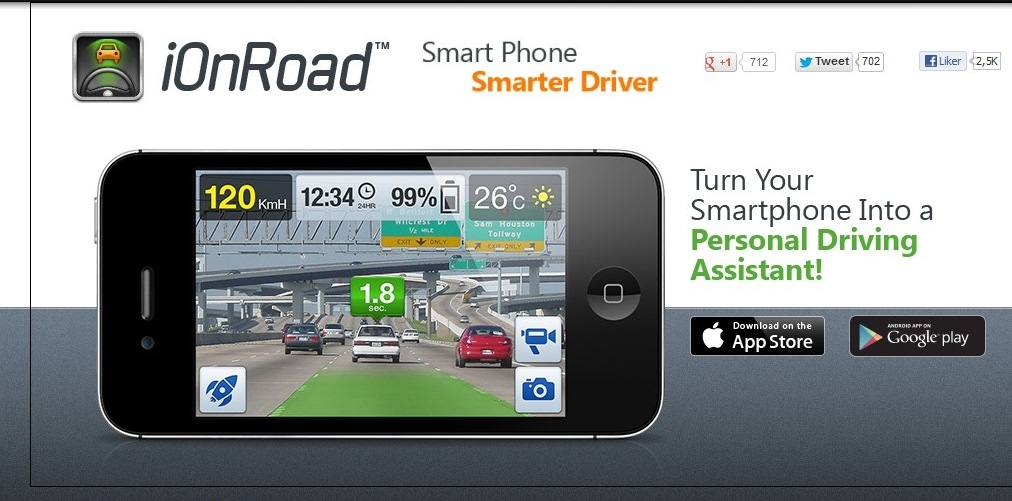
\includegraphics[scale=0.10]{img/iOnRoad.jpg}
\label{fig:iOnRoad1}
\end{figure}

\paragraph{Appen har en "Car-locator"-funksjon men med en liten twist i forhold til andre apper; den husker hvor bilen står parkert ved hjelp av GPS-lokasjonen. Deretter plasserer en markør på kartet, slik at når du skal finne bilen din igjen gjøres det ved hjelp av den lagrede GPS-dataen. I tillegg til dette finnes også en automatisk kjøringsdetektor som oppdager når sjåføren entrer bilen, og på denne måten blir Appen aktivert.}

\paragraph{Appen ble lansert i 2011 av en Israelsk selskap, og i startfasen var den kun tilgjengelig der. Men etter hvert ble den lansert internasjonalt, og er nå laste ned over 200 000 ganger. Appen har mottatt en god del priser, blant annen innen design og innovasjon.}

\begin{figure}[p]
\centering
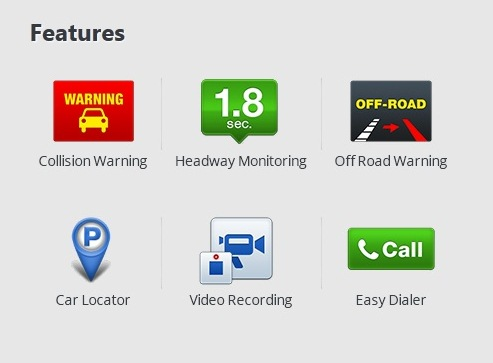
\includegraphics[scale=0.10]{img/iOnRoad2.jpg}
\caption{Funksjoner som tilbys}
\label{fig:iOnRoad2}
\end{figure}

\paragraph{iOnRoad er en app som tilbyr mange interessante funksjoner som du normalt ikke finner i vanlige GPS-applikasjoner. Deriblant kollisjonsvarsling, "black-box" varsling, lokasjon og bensinpriser. Flere brukere har testet denne applikasjoner og det ligger mye positiv tilbakemelding på nettet, i tillegg er gjennomsnittsvurdering på 4,2 (5 er høyest).}


\subsection{Google Maps}

\paragraph{Google Maps kan beskrives som standarden innen kart løsninger, særlig på internett. Tjenesten eksisterer både som en web- løsning og som apper til de fleste mobile plattformer som finnes. Tilbyr i tillegg til kart et hav av funskjoner som ruteplanlegging med sving for sving navigasjon, visning av sanntidsdata, osv. Noen av dem er beskrevet nedenfor.}

\paragraph{En av funksjonen vi la spesielt merke til er muligheten for å vise sanntidsinformasjon fra trafikken. Google Maps viser trafikkmengden ved hjelp av fargekoder langs strekningen, og viser også eventuelle hindringer langs veien. Tjenesten tar hensyn til denne informasjonen når den regner ut hvilen rute som vil være raskest. I tillegg bruker den informasjonen til å estimere drivstofforbruk, ved å ta hensyn til rute, trafikkmengde og biltype.}

\begin{figure}[p]
\centering
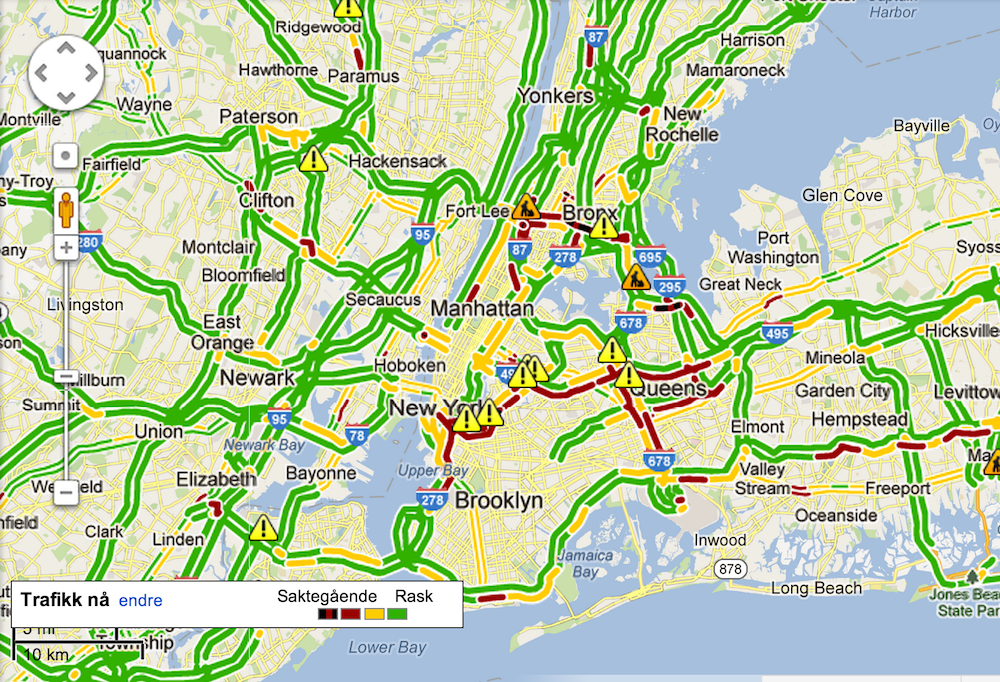
\includegraphics[scale=0.10]{img/google_maps1.jpg}
\caption{Et eksempel på sanntidsdata hentet fra New York. Gir informasjon om trafikkmengde, ulykker, veiarbeid, osv.}
\label{fig:google_maps1}
\end{figure}

\paragraph{Sanntidsdataen blir hentet ved hjelp av anonym innsamling fra GPS enheter som bruker veiene(en form for crowdsourcing). Google et enormt brukergrunnlag tilgjengelig ved hjelp av Google Maps applikasjon til Android og iOS enheter. Sanntidsdata fra trafikken er kun utbredt tilgjengelig i de største landene som USA, Frankrike og Storbritannia. Nye land og byer legges til fortløpende. Sanntidsdata vises også i norske byer, men dette gjelder et veldig begrenset antall strekninger, og informasjonen virker ikke å være spesielt nøyaktige.}

\paragraph{Google Maps bruker denne dataen til å foreslå den raskeste ruten. I denne utregningen inngår både sanntidsdata og historiske data(elementer av intelligente metoder) til å estimere trafikkmengden. Når man planlegger en rute får man dermed opp flere alternativer sortert etter estimert tid.}

\begin{figure}[p]
\centering
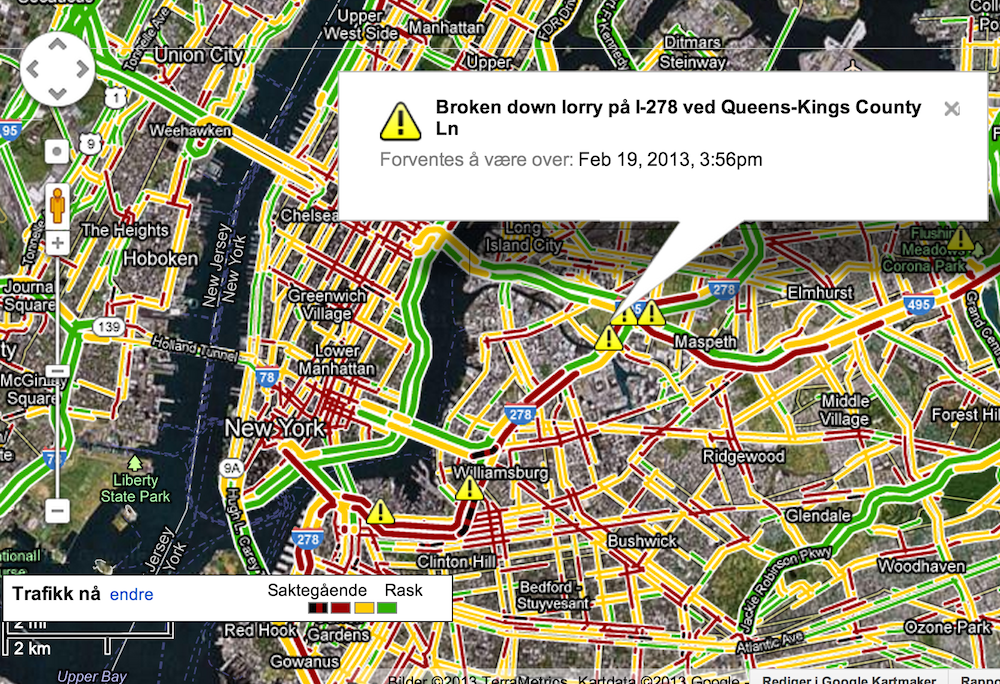
\includegraphics[scale=0.10]{img/google_maps2.jpg}
\caption{Google Maps gir også detaljert informasjon om hindringer i trafikken}
\label{fig:google_maps2}
\end{figure}

\paragraph{Google Maps tilbyr mange spennende funskjoner som kan lett kan tenkes å være en del av et intelligent trafikksystem. Spesielt integreringen av sanntidsdata og hvordan denne blir brukt er interessant for oss. Selv om mesteparten av disse funskjonene ikke er tilgjengelig i Norge, viser det oss at det er teknisk mulig å implementere de og gir oss tips om hvordan(crowdsourcing).}


\subsection{Waze}
\paragraph{Waze er laget av et israelsk selskap og er en meget populær app som brukes over hele verden, men hovedsaklig i USA. . Den har for tiden rundt 30 millioner brukere. All informasjon som leveres til brukeren er generert av andre brukere(crowdsourcing). Dette gjøres via en applikasjon til smarttelefoner, der man har mulighet til å rapportere ulike type hendelser, som f.eks. ulykker, fareelementer i veien og køer. Disse rapportene blir knyttet til veistrekningen man er på til en hver tid, og brukes til å advare andre trafikanter. Selve kartet oppdateres også ved hjelp av brukerne, slik at de til en hver tid er oppdatert.}

\paragraph{Waze genererer både automatiske rapporter med bakgrunn i bevegelsene til brukeren og manuelle rapporter som er lagt inn av brukere. De automatiske rapportene genereres ved å f.eks. overvåke brukerens hastighet. Hvis man registrerer at brukeren forflytter seg saktere enn den gjeldende fartsgrensen på veien, vil det genereres en rapport om kø i dette området. Man har mulighet for å gi tilbakemelding på rapporter fra andre brukere, ved å enten godkjenne dem eller gi beskjed om at problemet ikke lenger er der. På denne måten vil trafikkmeldingene til en hver tid være oppdatert.}

\begin{figure}[p]
\centering
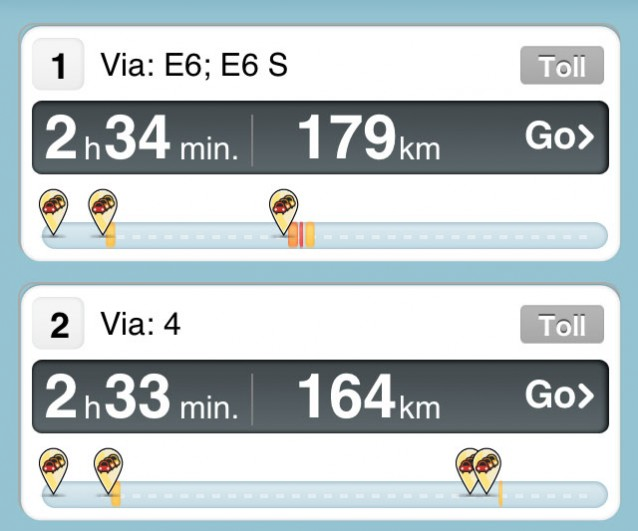
\includegraphics[scale=0.10]{img/waze1.jpg}
\label{fig:waze1}
\end{figure}

\paragraph{Waze har også mulighet til å sammenligne forskjellige ruter til en bestemt destinasjon. Den vil ta hensyn til rapporter om f.eks. kø og gi et estimat om hvor lang tid hver strekning vil ta. Waze har også innslag av intelligente funksjoner. Tjenesten tar vare på dine tidligere bevegelser og lærer etterhvert hvor du vanligvis kjører. Avhengig av tidspunkt og posisjon vil man etterhvert få opp forslag om hvor man vil kjøre når man starter appen(context awareness, læringsalgoritme).}

\begin{figure}[p]
\centering
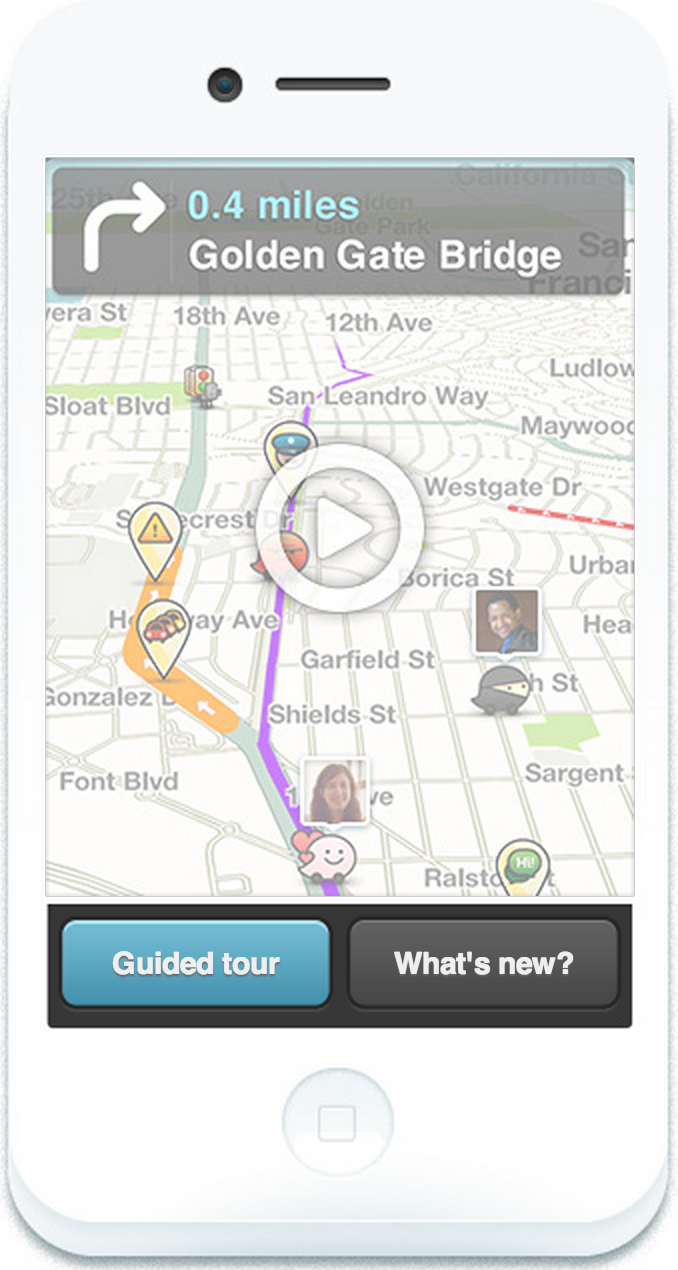
\includegraphics[scale=0.10]{img/waze2.jpg}
\label{fig:waze2}
\end{figure}

\paragraph{Waze tilbyr begrenset funksjonalitet i Norge som følge av at det ikke finnes så mange brukere her(Begynner å ta seg opp, spesielt i Oslo. \footnote{http://nrkbeta.no/2013/02/25/waze-revolusjonerende-bilnavigering/#more-23895} Nettopp premiert som “Best Overall Mobile App” på Global Mobile Awards i Barcelona.}


\subsection{Ras}
\paragraph{Vi har forsøkt å finne løsninger i utlandet som kan vise rasfare langs en veistrekning uten å lykkes. Det finnes mange lokale informasjonssystemer, noen med tilhørende applikasjoner, som informerer om rasfare i spesielle områder. Dette gjelder helst snøskred og som oftest i forbindelse med skisentre. I tillegg virker som om de fleste av disse løsningene fokuserer på å oppgi risiko for ras i visse områder, og ikke informasjon om når det har gått et ras.}

\subsection{Veiforhold}
\paragraph{Det finnes noen eksempler i utlandet på apper som kan vise informasjon om veiforhold. Men dette er som oftest tilgjengelig i et begrenset område, og de få eksemplene vi har funnet er knyttet til visse stater i USA. Ut i fra det vi kan finne henter disse løsningene gjerne informasjon fra offisielle kilder innad i staten. Virker ikke som om det finnes et sentralt system for hele USA.}



